%  The AAU Poster Theme.
%  2013-05-08 v. 1.1.0
%  Copyright 2013 by Jesper Kjær Nielsen <jkn@es.aau.dk>
%
%  This is free software: you can redistribute it and/or modify
%  it under the terms of the GNU General Public License as published by
%  the Free Software Foundation, either version 3 of the License, or
%  (at your option) any later version.
%
%  This is distributed in the hope that it will be useful,
%  but WITHOUT ANY WARRANTY; without even the implied warranty of
%  MERCHANTABILITY or FITNESS FOR A PARTICULAR PURPOSE.  See the
%  GNU General Public License for more details.
%
%  You can find the GNU General Public License at <http://www.gnu.org/licenses/>.
% http://www.brian-amberg.de/uni/poster/baposter/baposter_guide.pdf

\documentclass[paperwidth=78cm,paperheight=110cm,portrait]{baposter}
% paper= portrait, %landscape,
%paper= 110cm:78cm, almost like a0paper
%%%%%%%%%%%%%%%%%%%%%%%%%%%%%%%%%%%%%%%%%%%%%%%%
% Language, Encoding and Fonts
% http://en.wikibooks.org/wiki/LaTeX/Internationalization
%%%%%%%%%%%%%%%%%%%%%%%%%%%%%%%%%%%%%%%%%%%%%%%%
% Select encoding of your inputs. Depends on
% your operating system and its default input
% encoding. Typically, you should use
%   Linux  : utf8 (most modern Linux distributions)
%            latin1 
%   Windows: ansinew
%            latin1 (works in most cases)
%   Mac    : applemac
% Notice that you can manually change the input
% encoding of your files by selecting "save as"
% an select the desired input encoding. 

\usepackage{outlines}
\usepackage{soul} % for \underline{}
\usepackage{tabularx} % for resizebox?
\usepackage{colortbl}     % arrayrulecolor
\usepackage{multirow}
\usepackage{siunitx} % for  1e-10 scientific notation, \num
\usepackage[backend=biber,style=authoryear,citestyle=authoryear]{biblatex}
% \parencite{Saussure1995}
\renewcommand*{\nameyeardelim}{\addcomma\addspace}
\addbibresource{TCGA_margin_cutoff.bib}
%% TCGA_margin_cutoff.bib
%%%%
%%% for abbreviations, or acronyms
\usepackage[acronym, nopostdot]{glossaries}  % automake
\usepackage{glossary-inline}
%\setacronymstyle{long-short}
%\renewcommand*{\glossarysection}[2][]{} 
%\renewcommand*{\glossarysection}[2][]{\textbf{#1}: }
% for abbreviations environment
%\newcommand{\abbrlabel}[1]{\makebox[3cm][l]{\textbf{#1}\ \dotfill}}
\newenvironment{abbreviation}


%\section{abbreviation}
%%%%%%%%%%%%% Define abbreviation
%\makeglossaries %https://tex.stackexchange.com/questions/110095/list-of-acronyms-is-not-displayed



\newacronym{ncbi}{NCBI}{National Center for Biotechnology Information}
\newacronym{degs}{DEGs}{differentially expressed genes}

\newacronym{ihc}{IHC}{immunohistochemistry}
\newacronym{fdr}{FDR}{false discovery rate}

\newacronym{hpa}{HPA}{the Human Protein Atlas}
\newacronym{hnscc}{HNSCC}{head and neck squamous cell carcinoma}
\newacronym{tcga}{TCGA}{the Cancer Genome Atlas}
\newacronym{tcpa}{TCPA}{the Cancer Proteome Atlas}
\newacronym{rna}{RNA}{ribonucleic acid}
\newacronym{rnaseq}{RNA-Seq}{RNA sequencing}
\newacronym{lncrna}{lncRNA}{long non-coding RNA}
%\newacronym{km}{KM}{Kaplan--Meier}
\newacronym{rppa}{RPPAs}{reverse-phase protein arrays}
\newacronym{rpma}{RPMA}{reverse-phase protein lysate microarray}

\newacronym{mmp}{MMP}{matrix metalloproteinase}
 %DKK1, CAMK2N1, STC2, PGK1, SURF4, USP10, NDFIP1, FOXA2, STIP1, and DKC1
 %ZNF557, ZNF266, IL19, MYO1H, FCGBP, LOC148709, EVPLL, PNMA5, KIAA1683, and NPB

\newacronym{DKK1}{DKK1}{dickkopf WNT signaling pathway inhibitor 1} 
\newacronym{CAMK2N1}{CAMK2N1}{calcium/calmodulin dependent protein kinase II inhibitor 1} 
\newacronym{CALML5}{CALML5}{calmodulin like 5}

\newacronym{STC2}{STC2}{stanniocalcin 2} 
\newacronym{PGK1}{PGK1}{phosphoglycerate kinase 1} 
\newacronym{SURF4}{SURF4}{surfeit 4} 
\newacronym{USP10}{USP10}{ubiquitin specific peptidase 10} 
\newacronym{NEDD4}{NEDD4}{neural precursor cell expressed, developmentally down-regulated 4}
\newacronym{NDFIP1}{NDFIP1}{NEDD4 family interacting protein 1} 
\newacronym{FOXA2}{FOXA2}{forkhead box A2} 
\newacronym{STIP1}{STIP1}{stress-induced-phosphoprotein 1} 
\newacronym{DKC1}{DKC1}{dyskeratosis congenita 1, dyskerin} 

\newacronym{ZNF557}{ZNF557}{zinc finger protein 557} 
\newacronym{ZNF266}{ZNF266}{zinc finger protein 266} 
\newacronym{IL19}{IL19}{interleukin 19} 
\newacronym{MYO1H}{MYO1H}{myosin 1H} 
\newacronym{FCGBP}{FCGBP}{Fc fragment of IgG binding protein} 
\newacronym{LOC148709}{LOC148709}{LncRNA LOC148709} 
\newacronym{EVPLL}{EVPLL}{envoplakin-like protein} 
\newacronym{PNMA5}{PNMA5}{paraneoplastic antigen like 5} 
%\newacronym{KIAA1683}{KIAA1683}{IQCN, IQ Motif Containing N} 
\newacronym{IQCN}{IQCN}{IQ motif containing N} % previous name KIAA1683
% "IQ'' refers to the first two amino acids of the motif: isoleucine (commonly) and glutamine (invariably)
\newacronym{NPB}{NPB}{neuropeptide B} 

 \newacronym{rt}{RT}{radiation therapy}
 \newacronym{nccn}{NCCN}{National Comprehensive Cancer Network}
 \newacronym{hif}{HIF}{hypoxia-inducible factor}
 \newacronym{egfr}{EGFR}{epidermal growth factor receptor}
 \newacronym{ras}{RAS}{rat sarcoma}
 \newacronym{hras}{HRAS}{Harvey rat sarcoma viral oncoprotein}
 \newacronym{erk}{ERK}{extracellular signal-regulated kinases}
 \newacronym{us}{US}{United States}
 \newacronym{fda}{FDA}{Food and Drug Administration}
 \newacronym{tpf}{Tax-PF}{docetaxel, cisplatin, and 5-fluorouracil}
 \newacronym{tki}{TKI}{tyrosine kinase inhibitor}
 \newacronym{her}{HER}{human epidermal growth factor receptor}
 \newacronym{ici}{ICI}{immune-checkpoint inhibitor}
 \newacronym{ctla4}{CTLA-4}{cytotoxic T lymphocyte antigen 4}
 \newacronym{pd1}{PD-1}{programmed death 1}
 \newacronym{pdl1}{PD-L1}{programmed death ligand 1}
 \newacronym{tim3}{TIM-3}{T-cell immunoglobulin mucin protein 3}
 \newacronym{lag3}{LAG-3}{lymphocyte activation gene 3}
 \newacronym{ifng}{IFN-$\gamma$}{interferon gamma}
 \newacronym{tigit}{TIGIT}{T cell immunoglobin and immunoreceptor tyrosine-based inhibitory motif}
 \newacronym{gitr}{GITR}{glucocorticoid-induced tumor necrosis factor receptor}
 \newacronym{vista}{VISTA}{V-domain Ig suppressor of T-cell activation}
 \newacronym{tmsb4x}{TMSB4X}{thymosin beta-4 X-linked}
 \newacronym{emt}{EMT}{epithelial-mesenchymal-transition}
 \newacronym{gdc}{GDC}{Genomic Data Commons}
 \newacronym{nci}{NCI}{the National Cancer Institute}
 \newacronym{gdac}{GDAC}{genome data analysis center}
 \newacronym{rest}{REST}{Representational State Transfer} 
 \newacronym{api}{API}{application programmable interface}
\newacronym{grch38}{GRCh38}{Genome Reference Consortium Homo sapiens genome assembly 38}
\newacronym{fpkm}{FPKM}{Fragments per kilobase per million reads mapped}
\newacronym{rsem}{RSEM}{RNA-Seq by Expectation-Maximization}
\newacronym{slca}{SLC35E2A}{solute carrier family 35 member E2A}
\newacronym{slcb}{SLC35E2B}{solute carrier family 35 member E2B}
\newacronym{cde}{CDE}{Common Data Element}
\newacronym{id}{ID}{identification}
\newacronym{ajcc}{AJCC}{the American Joint Committee on Cancer}
\newacronym{uicc}{UICC}{he Union for International Cancer Control}
\newacronym{tnm}{TNM}{the tumor size (T), cervical lymph node metastases (N), and distal metastasis status (M)}
\newacronym{ci95}{95\% CI}{95\% confidence interval}
\newacronym{os}{OS}{overall survival}
\newacronym{hr}{HR}{hazard ratio}
\newacronym{hpv}{HPV}{human papillomavirus}
\newacronym{ene}{ENE}{extra-nodal extension}
\newacronym{lvsi}{LVSI}{lymph-vascular space invasion}
\newacronym{pni}{PNI}{perineural invasion}
\newacronym{doi}{DOI}{depth of invasion}
\newacronym{lnd}{LND}{lymph node density}
\newacronym{wpoi5}{WPOI-5}{worst pattern of invasion score 5}
\newacronym{glut4}{GLUT4}{glucose transporter 4}
\newacronym{slc2a4}{SLC2A4}{solute carrier family 2 member A4}
\newacronym{trim24}{TRIM24}{tripartite motif-containing 24}
\newacronym{til}{TIL}{tumor-infiltrating lymphocytes}
\newacronym{tmb}{TMB}{tumor mutational burden}



%%
\usepackage[utf8]{inputenc}
% Make latex understand and use the typographic
% rules of the language used in the document.
\usepackage[english]{babel}
% Use the vector font Latin Modern which is going
% to be the default font in latex in the future.
\usepackage{helvet}
% Change the default font family from roman to sans serif
\renewcommand{\familydefault}{\sfdefault} % for text
\usepackage[helvet]{sfmath} % for math
% Choose the font encoding
\usepackage[T1]{fontenc}

%%%%%%%%%%%%%%%%%%%%%%%%%%%%%%%%%%%%%%%%%%%%%%%%
% Graphics and Tables
% http://en.wikibooks.org/wiki/LaTeX/Importing_Graphics
% http://en.wikibooks.org/wiki/LaTeX/Tables
% http://pgfplots.sourceforge.net/
%%%%%%%%%%%%%%%%%%%%%%%%%%%%%%%%%%%%%%%%%%%%%%%%
% You cannot use floats in the baposter theme.
% We therefore load the caption package which provides
% the command \captionof
% Set up how figure and table captions are displayed
\usepackage{caption}
\captionsetup{
  font=small,% set font size to footnotesize
  labelfont=bf % bold label (e.g., Figure 3.2) font
}
% Make the standard latex tables look so much better
\usepackage{array,booktabs}
% For creating beautiful plots
\usepackage{pgfplots}

%%%%%%%%%%%%%%%%%%%%%%%%%%%%%%%%%%%%%%%%%%%%%%%%
% Mathematics
% http://en.wikibooks.org/wiki/LaTeX/Mathematics
%%%%%%%%%%%%%%%%%%%%%%%%%%%%%%%%%%%%%%%%%%%%%%%%
% Defines new environments such as equation,
% align and split 
\usepackage{amsmath}
% Adds new math symbols
\usepackage{amssymb}

%%%%%%%%%%%%%%%%%%%%%%%%%%%%%%%%%%%%%%%%%%%%%%%%
% Colours
% http://en.wikibooks.org/wiki/LaTeX/Colors
%%%%%%%%%%%%%%%%%%%%%%%%%%%%%%%%%%%%%%%%%%%%%%%%
\selectcolormodel{RGB}
% define the three aau colors
\definecolor{aaublue1}{RGB}{33,26,82}% dark blue
\definecolor{aaublue2}{RGB}{113,109,143} % light blue
\definecolor{aaublue3}{RGB}{194,193,204} % lighter blue

%%%%%%%%%%%%%%%%%%%%%%%%%%%%%%%%%%%%%%%%%%%%%%%%
% Lists
% http://en.wikibooks.org/wiki/LaTeX/List_Structures
%%%%%%%%%%%%%%%%%%%%%%%%%%%%%%%%%%%%%%%%%%%%%%%%
% Easier configuration of lists
\usepackage{enumitem}
%configure itemize
\setlist{%
  topsep=0pt,% set space before and after list
  noitemsep,% remove space between items
  labelindent=\parindent,% set the label indentation to the paragraph indentation
  leftmargin=*,% remove the left margin
  font=\color{aaublue1}\normalfont, %set the colour of all bullets, numbers and descriptions to aaublue1
}
% use set<itemize,enumerate,description> if you have an older latex distribution
\setitemize[1]{label={\raise1.25pt\hbox{$\blacktriangleright$}}}
\setitemize[2]{label={\scriptsize\raise1.25pt\hbox{$\blacktriangleright$}}}
\setitemize[3]{label={\raise1.25pt\hbox{$\star$}}}
\setitemize[4]{label={-}}
%\setenumerate[1]{label={\theenumi.}}
%\setenumerate[2]{label={(\theenumii)}}
%\setenumerate[3]{label={\theenumiii.}}
%\setenumerate[4]{label={\theenumiv.}}
%\setdescription{font=\color{aaublue1}\normalfont\bfseries}

% use setlist[<itemize,enumerate,description>,<level>] if you have a newer latex distribution
%\setlist[itemize,1]{label={\raise1.25pt\hbox{$\blacktriangleright$}}}
%\setlist[itemize,2]{label={\scriptsize\raise1.25pt\hbox{$\blacktriangleright$}}}
%\setlist[itemize,3]{label={\raise1.25pt\hbox{$\star$}}}
%\setlist[itemize,4]{label={-}}
%\setlist[enumerate,1]{label={\theenumi.}}
%\setlist[enumerate,2]{label={(\theenumii)}}
%\setlist[enumerate,3]{label={\theenumiii.}}
%\setlist[enumerate,4]{label={\theenumiv.}}
%\setlist[description]{font=\color{aaublue1}\normalfont\bfseries}

%%%%%%%%%%%%%%%%%%%%%%%%%%%%%%%%%%%%%%%%%%%%%%%%
% Misc
%%%%%%%%%%%%%%%%%%%%%%%%%%%%%%%%%%%%%%%%%%%%%%%%
% change/remove some names
\addto{\captionsenglish}{
  %remove the title of the bibliograhpy
  \renewcommand{\refname}{\vspace{-0.7em}}
  %change Figure to Fig. in figure captions
  \renewcommand{\figurename}{Fig.}
}
% create links
\usepackage{url}
%note that the hyperref package is currently incompatible with the baposter class

%%%%%%%%%%%%%%%%%%%%%%%%%%%%%%%%%%%%%%%%%%%%%%%%
% Macros
%%%%%%%%%%%%%%%%%%%%%%%%%%%%%%%%%%%%%%%%%%%%%%%%
\newcommand{\alert}[1]{{\color{aaublue1}#1}}

%%%%%%%%%%%%%%%%%%%%%%%%%%%%%%%%%%%%%%%%%%%%%%%%
% Document Start 
%%%%%%%%%%%%%%%%%%%%%%%%%%%%%%%%%%%%%%%%%%%%%%%%
\begin{document}
%%%%%%%%%%%%%%%%%%%%%%%%%%%%%%%%%%%%%%%%%%%%%%%%
% Some changes that cannot be made in the preamble
%%%%%%%%%%%%%%%%%%%%%%%%%%%%%%%%%%%%%%%%%%%%%%%%
% set the background of the poster
\background{
  \begin{tikzpicture}[remember picture,overlay]%
    %the poster background color
    \fill[fill=aaublue3] (current page.north west) rectangle (current page.south east);
    %the header
    \fill [fill=aaublue1] (current page.north west) rectangle ([yshift=-\headerheight] current page.north east);
  \end{tikzpicture}
}
% if you want to reduce the space before and after equations, use and adjust
% the following lines
%\addtolength{\abovedisplayskip}{-2mm}
%\addtolength{\belowdisplayskip}{-2mm}

%%%%%%%%%%%%%%%%%%%%%%%%%%%%%%%%%%%%%%%%%%%%%%%%
% General poster setup
%%%%%%%%%%%%%%%%%%%%%%%%%%%%%%%%%%%%%%%%%%%%%%%%
\begin{poster}{
  %general options for the poster
  grid=false,
  columns=3,
%  colspacing=4.2mm,
  headerheight=0.1\textheight,
  background=user,
%  bgColorOne=red!42, %is used when background != user and none
%  bgColortwo=green!42, %is used when background is shaded
  eyecatcher=true,
  %posterbox options
  headerborder=closed,
  borderColor=aaublue1,
  headershape=rectangle,
  headershade=plain,
  headerColorOne=aaublue1,
%  headerColortwo=yellow!42, %is used when the header background is shaded
  textborder=rectangle,
  boxshade=plain,
  boxColorOne=white,
%  boxColorTwo=cyan!42,%is used when the text background is shaded
  headerFontColor=white,
  headerfont=\Large\sf\bf,
  linewidth=1pt
}
%the Eye Catcher (the logo on the left)
{
  %this can be commented out or replaced by a company/department logo
  
\includegraphics[height=0.75\headerheight]{TMU_TMWH_logo.pdf} %{https://www.tmu.edu.tw/images/title.png}
}
%the poster title
{\color{white}\bf
  \Large A Transcriptomic Analysis of Head and Neck Squamous Cell Carcinomas for Prognostic Indications
}
%the author(s)
{\color{white}\small
  \vspace{1em} Li-Hsing (Tex) Chi, D.D.S, Ph.D. Candidate \\[0.5em] % Jesper Kjær Nielsen
  Oral and Maxillofacial Surgery \\
  Dept.\ of Dentistry, Wan Fang Hospital, Taipei Medical University, Taipei, Taiwan\\
  110050@w.tmu.edu.tw
}
%the logo (the logo on the right)
{
%  Video Abstract:
  
\includegraphics[height=0.65\headerheight]{QRcode_VideoAbstract_JPM-1309345.pdf}
}



%------------------------------------------------
%%%%%%%%%%%%%%%%%%%%%%%%%%%%%%%%%%%%%%%%%%%%%%%%
% the actual content of the poster begins here
%%%%%%%%%%%%%%%%%%%%%%%%%%%%%%%%%%%%%%%%%%%%%%%%
\section{Introduction}


\begin{posterbox}[name=intro,column=0,row=0]{Introduction}


\begin{outline}
    \1 Survival analysis of \acrfull{tcga} dataset for \acrfull{hnscc}
        \2 gene expression-based prognostic biomarkers
        \2 a \underline{cutoff} point (Fig.\ref{fig:workflow}) is usually used in survival analysis
%hl{} is not working

\0 The advantages of applying the TCGA data for cancer biomarker identification include:
\1  the TCGA database has the \underline{largest collection} (cancer types and cohort size), especially in HNSCC)
%There are many physical and social features of patients available for survival modeling. % ($X_1 ... X_n$)
\2 the whole-genome sequencing data were harmonized
\2 the essential demographic data, physical and social features of patients (exposure to alcohol, asbestos, radioactive radon, \underline{tobacco} smoking, and cigarettes)
%\2 computational and life scientists who study cancer designed useful web-based tools and APIs (\footnotesize Application Programming Interface---program talks to program)
\1 getting \underline{help} soon from the research community for trouble-shooting purposes
%\1 many achievements and getting published, including \underline{Chi} et al., 2021~\cite{Chi2021}.
\1 "an immeasurable source of knowledge"~[Tomczak, 2015]   %\cite{Tomczak2015}
\1 The results were published[Chi, 2021] (at \url{https://www.mdpi.com/2075-4426/11/8/782/htm}) and shown here are in part based upon data generated by the TCGA Research Network: \url{https://www.cancer.gov/tcga}.
\end{outline}
\begin{center}
% QR code
\footnotesize Full article available (scan me):

\includegraphics[width=0.3\textwidth]{QRcode_JPM-1309345.png}
\end{center}
\end{posterbox}

%%%
\section{Materials and Methods}
\begin{posterbox}[name=lists,column=0,below=intro, ,above=bottom]{Materials and Methods}

\begin{outline}

\begin{center}
    \includegraphics[width=0.9\textwidth]{Figure_1_manuscript_workflow_modify.pdf}
    \captionof{figure}{An in-house workflow---pvalueTex}
    \label{fig:workflow}
\end{center}   
%    \0 An in-house workflow---pvalueTex
        \1 data retrieving from TCGA via FirebrowseR package
            \2 data cleaning
            \2 feature selection
        \1 \underline{sliding-window} cutoff mining engine for Kaplan--Meier survival analysis to find a optimal cutoff
        \1 Cox proportional hazard modeling~[Cox, 1972][Bradburn, 2003]\: % Andersen1982,
        %Here is an example of an equation
%\begin{equation}
%  f_X(x|\mu,\sigma^2) = \frac{1}{\sqrt{2\pi\sigma^2}}\exp\left\{\frac{1}{2\sigma^2}(x-\mu)^2\right\}
%\end{equation}
$$h(t) = h_0(t) \times e^{(\beta_1 X_1 + \beta_2 X_2 + \beta_3 X_3 + ... + \beta_n X_n)}$$
%$$h(t) = h_0(t) \times exp(\beta_1 X_1 + \beta_2 X_2 + \beta_3 X_3 + ... + \beta_n X_n)$$
% natural exponential function => y=e^x
%\end{flushleft}
%\noindent where,
%\begin{outline} % for highlight
%\1 $t$ represents the survival time;
%\1 $h(t)$ is the hazard function determined by a set of n covariates ($X_1...X_n$)---e.g., clinicopathological features
%\1 The coefficients ($\beta_1...\beta_n$) measure the impacts---\underline{the effect sizes} (i.e., hazard ratios) of covariates;
%\1 e is the Euler's number;
%\1 The term $h_0$ is called the baseline hazard.
%\1 A collection of $X_1...X_n$ features from cancer datasets
%\end{outline}
        \1 validation by (GSE65858)~[Ichmann, 2015]
\end{outline}
\end{posterbox}
%

%\begin{posterbox}[name=equation,column=0,below=lists,above=bottom]{Equations}

%\end{posterbox}

\section{Results}

\begin{posterbox}[name=install,span=2,column=1,row=0]{Results}
The way to find our biomarkers: CAMK2N1, CALML5, and FCGBP.
\end{posterbox}\\
 FDR then Bonferroni\\
 


%%
\begin{posterbox}[name=figures,column=1,below=install,above=bottom]{Figures and Tables}

\begin{center}
  \includegraphics[width=0.9\textwidth]{Figure_4_CAMK2N1_CALML5_FCGBP.pdf}
  \label{fig:3KM}
  \captionof{figure}{
During \underline{cutoff finding} (within 30\%--70\% quantile), hundreds of Kaplan--Meier (KM) plots were generated for each gene.\\
- The cutoffs (gene expression) were shown in the cumulative FDR-adjusted \underline{\textit{p}~value plots} of  CAMK2N1, CALML5, and FCGBP.\\
- The KM curves of CAMK2N1, CALML5, and FCGBP with \underline{optimal \textit{p}~values}.\\
%((b) the cutoffs derived from it's cumulative \protect\textit{p}~value plot).
%(c) Kaplan--Meier plot of IL19 under optimal \protect\textit{p}~value;
%((d) the cutoffs derived from it's cumulative \protect\textit{p}~value plot).
%(e) Kaplan--Meier plot of FCGBP under optimal \protect\textit{p}~value.\\
%The optimal cutoff value for CAMK2N1 is 
%,
%show that over 50\% of those unadjusted \protect\textit{p}~values derived by the sliding-window cutoff-finding procedure are below 0.001.
\footnotesize (\protect\textit{p}~value adjusted by \acrlong{fdr}, \acrshort{fdr})
}
%  \label{fig:figlabel}
\end{center}

%
\begin{center}
%    \begin{table}[] 
%\centering
%\caption{The top 3 genes with prognostic impacts on HNSCC.}% (ranked by Bonferroni-adjusted \protect\textit{p}~values}

%%%\label{tab:newTable1}
\resizebox{1\linewidth}{!}{% \textwidth
\begin{tabular}{|l|l|l|c|c|c|c|c|c|}
\noalign{\hrule height 1.0pt}
\multicolumn{1}{|c|}{} &
  \multicolumn{2}{c|}{} &
  \multicolumn{2}{c|}{\textbf{Kaplan--Meier Survival}} &
  \multicolumn{2}{c|}{\textbf{Cox Univariate}} &
  \multicolumn{2}{c|}{\textbf{Cox Multivariate}} \\ \cline{4-9} 
\multicolumn{1}{|l|}{\multirow{-2}{*}{\textbf{Gene ID}}} &
  \multicolumn{2}{l|}{\multirow{-2}{*}{\textbf{Gene Descriptio}n}} &
  \begin{tabular}[c]{@{}c@{}}\textbf{FDR}\\ \textbf{\protect\textit{p}~Value}\end{tabular} &
  \begin{tabular}[c]{@{}c@{}}\textbf{Bonferroni}\\ \textbf{\protect\textit{p}~Value}\end{tabular} &
  \textbf{HR *} &
  \textbf{CI95\%} &
  \textbf{HR *} &
  \textbf{CI95\%} \\ 
  \underlineine
CAMK2N1 &
  \multicolumn{2}{l|}{\begin{tabular}[c]{@{}l@{}}calcium/calmodulin-\\ dependent protein\\ kinase II inhibitor 1\end{tabular}} &
  \num{1.63e-5} & %2.9e-7} &
  0.002 &
  2.101 &
  1.572--2.809 &
  2.007 &
  1.490--2.704 \\ \underlineine
CALML5 &
  \multicolumn{2}{l|} {\acrlong{CALML5}} &
   \num{1.97e-4} & %\num{6.54e-6} & %3.7e-7} &
   0.039 &
   0.51 &
   0.379--0.686 &
   0.493 &
   0.364--0.667 \\ \underlineine
FCGBP &
  \multicolumn{2}{l|}{\begin{tabular}[c]{@{}l@{}}Fc fragment of\\  IgG binding protein\end{tabular}} &
   \num{4.83e-5} & %1.2e-6} &
   0.008 &
   0.484 &
   0.359--0.653 &
   0.496 &
   0.366--0.674 \\ 
\noalign{\hrule height 1.0pt}
%\multicolumn{9}{|l|}{} \\
%\multicolumn{9}{|l|}%{\multirow{-0}{*}
%{\begin{tabular}[c]{@{}l@{}}
%
%\end{tabular}
%%}\\ % within \multirow
%} \\ % within \multicolumn
%\underlineine
%\multicolumn{9}{|l|}{ \\ \underlineine

\end{tabular}%
} % end of resizebox
%\pbox{0.8\columnwidth}{\footnotesize
%~\\
\captionof{table}{
The top 3 genes with prognostic impacts on HNSCC. Selection criteria (fit all):\\
(1) Kaplan--Meier Bonferroni-adjusted~\underline{\textit{p} \textless~0.05} in TCGA; \\
(2) Cox's univariate and multivariate \underline{HR \textgreater{}= 1.8 or \textless{}= 0.6} in both HNSCC (TCGA) and HNSCC (GSE65858) cohorts.\\
%(3) Cox's univariate and multivariate HR \textgreater{}= 1.8 or \textless{}= 0.6 in GSE65858 cohort.\\
*~Cox's model: \underline{\textit{p} \textless 0.001}
(HR: hazard ratio; CI95\%: 95\% confidence interval)
}

%\end{table}
\end{center}






%%%%%%%%%%
\begin{center}
    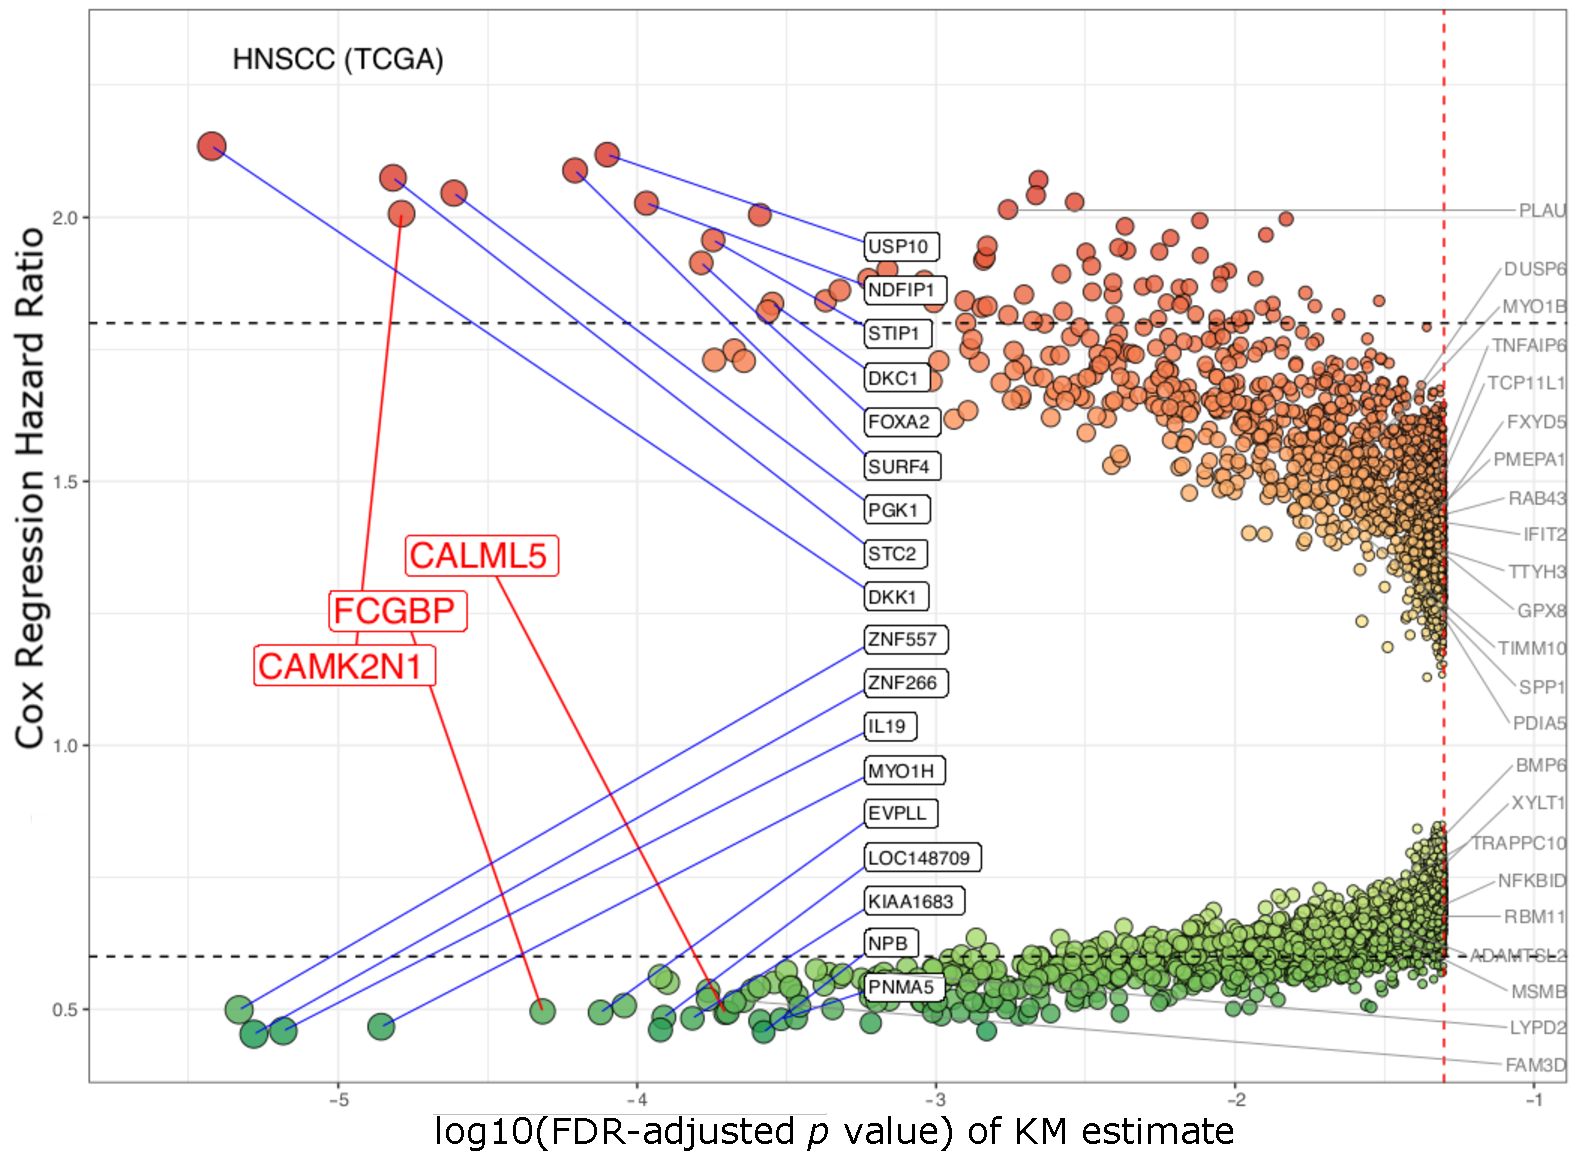
\includegraphics[width=0.95\textwidth]{Rplot_TCGA_HNSCC_CoxHR_CAMK2N1_top3FDRKM.pdf}
%{\captionsetup{labelformat=empty}    
\captionof{figure}{A volcano plot of candidate genes in \underline{HNSCC (TCGA)}.\\
    \textcolor{red}{Red spots}: HR > 1.0;
    \textcolor{green}{Green spots}: HR < 1.0;
    \textcolor{red}{Red dash line}: FDR \textit{p} = 0.05.\\
    \textcolor{red}{CAMK2N1}, \textcolor{red}{CALML5}, \textcolor{red}{FCGBP}, and  other 17 genes had \underline{hazard ratios (HRs)} >$1.8$ or <$0.6$ and \underline{Bonferroni-adjusted} KM \textit{p} values $< 0.05$.
    }
\end{center}




\end{posterbox}








%%%%%%%%%%%%%%%%%%%%%%%%%%%%%%%%
%%% CAMK2N1 %%%%%%
%%%%%%%%%%%%%%%%%%%%%%%%%%%%%%%

\begin{posterbox}[name=problems,column=2,below=install]{Discussion: CAMK2N1}

 
 \begin{center}
     \arrayrulecolor[rgb]{0.255,0.255,0.255}


\resizebox{0.95\linewidth}{!}{%
\begin{tabular}{|l|l|c|c|c|c|c|c|} 
\noalign{\hrule height 1.0pt}
%\begin{tabularx}{\textwidth}{|p{2.5cm}|l|l|l|l|l|l|l|} 
%\arrayrulecolor{black}\cline{1-2}
\arrayrulecolor[rgb]{0.255,0.255,0.255}
\cline{3-8}
\multicolumn{2}{|l!{\color{black}\vrule}}{\multirow{2}{*}{\textbf{Features}}}                                                          & \multicolumn{3}{c|}{\textbf{Univariate}}                                                                                                                                                                                                                & \multicolumn{3}{c|}{\textbf{Multivariate}}                                                                                                                                                                                                               \\ 
\cline{3-8}
\multicolumn{2}{|l!{\color{black}\vrule}}{}                                                                                   & \multicolumn{1}{l!{\color{black}\vrule}}{\textbf{HR}}                                   & \multicolumn{1}{c!{\color{black}\vrule}}{\textbf{CI95\%}}                              & \multicolumn{1}{l!{\color{black}\vrule}}{\textbf{\protect\textit{p}~Value}}                    & \multicolumn{1}{l!{\color{black}\vrule}}{\textbf{HR}}                                   & \multicolumn{1}{c!{\color{black}\vrule}}{\textbf{CI95\%}}                              & \multicolumn{1}{l!{\color{black}\vrule}}{\textbf{\protect\textit{p}~Value}}                     \\ 
\arrayrulecolor{black}\underlineine
\multirow{2}{*}{Gender}                 & \multicolumn{1}{l!{\color{black}\vrule}}{{\cellcolor[rgb]{0.62,0.812,0.878}}Female} & \multicolumn{1}{l!{\color{black}\vrule}}{{\cellcolor[rgb]{0.62,0.812,0.878}}1} & \multicolumn{1}{l!{\color{black}\vrule}}{{\cellcolor[rgb]{0.62,0.812,0.878}}} & \multicolumn{1}{l!{\color{black}\vrule}}{{\cellcolor[rgb]{0.62,0.812,0.878}}} & \multicolumn{1}{l!{\color{black}\vrule}}{{\cellcolor[rgb]{0.62,0.812,0.878}}1} & \multicolumn{1}{l!{\color{black}\vrule}}{{\cellcolor[rgb]{0.62,0.812,0.878}}} & \multicolumn{1}{l!{\color{black}\vrule}}{{\cellcolor[rgb]{0.62,0.812,0.878}}}  \\ 
\cline{2-8}
                                        & Male                                                                                & 1.157                                                                          & 0.843--1.587                                                                   & 0.367                                                                         & 1.076                                                                          & 0.767--1.510                                                                   & 0.671                                                                          \\ 
\arrayrulecolor[rgb]{0.255,0.255,0.255}\underlineine
\multirow{2}{*}{Age at diagnosis}       & {\cellcolor[rgb]{0.62,0.812,0.878}}$<=65y$                                             & {\cellcolor[rgb]{0.62,0.812,0.878}}1                                           & {\cellcolor[rgb]{0.62,0.812,0.878}}                                           & {\cellcolor[rgb]{0.62,0.812,0.878}}                                           & {\cellcolor[rgb]{0.62,0.812,0.878}}1                                           & {\cellcolor[rgb]{0.62,0.812,0.878}}                                           & {\cellcolor[rgb]{0.62,0.812,0.878}}                                            \\ 
\cline{2-8}
                                        & $>65y$                                                                                 & 1.329                                                                          & 0.990--1.784                                                                   & 0.058                                                                         & 1.391                                                                          & 1.025--1.888                                                                   & \textcolor{red}{0.034}                                                         \\ 
\underlineine
\multirow{2}{*}{\textcolor{red}{Clinical T Status}}      & {\cellcolor[rgb]{0.62,0.812,0.878}}T1+T2                                            & {\cellcolor[rgb]{0.62,0.812,0.878}}1                                           & {\cellcolor[rgb]{0.62,0.812,0.878}}                                           & {\cellcolor[rgb]{0.62,0.812,0.878}}                                           & {\cellcolor[rgb]{0.62,0.812,0.878}}1                                           & {\cellcolor[rgb]{0.62,0.812,0.878}}                                           & {\cellcolor[rgb]{0.62,0.812,0.878}}                                            \\ 
\cline{2-8}
                                        & T3+T4                                                                               & 1.409                                                                          & 1.028--1.931                                                                   & \textcolor{red}{0.033}                                                        & 1.982                                                                          & 1.048--3.745                                                                   & \textcolor{red}{0.035}                                                         \\ 
\underlineine
\multirow{2}{*}{Clinical N Status}      & {\cellcolor[rgb]{0.62,0.812,0.878}}N0                                               & {\cellcolor[rgb]{0.62,0.812,0.878}}1                                           & {\cellcolor[rgb]{0.62,0.812,0.878}}                                           & {\cellcolor[rgb]{0.62,0.812,0.878}}                                           & {\cellcolor[rgb]{0.62,0.812,0.878}}1                                           & {\cellcolor[rgb]{0.62,0.812,0.878}}                                           & {\cellcolor[rgb]{0.62,0.812,0.878}}                                            \\ 
\cline{2-8}
                                        & N1-3                                                                                & 1.185                                                                          & 0.890--1.577                                                                   & 0.246                                                                         & 1.145                                                                          & 0.801--1.636                                                                   & 0.457                                                                          \\ 
\underlineine
\multirow{2}{*}{Clinical M Status}      & {\cellcolor[rgb]{0.62,0.812,0.878}}M0                                               & {\cellcolor[rgb]{0.62,0.812,0.878}}1                                           & {\cellcolor[rgb]{0.62,0.812,0.878}}                                           & {\cellcolor[rgb]{0.62,0.812,0.878}}                                           & {\cellcolor[rgb]{0.62,0.812,0.878}}1                                           & {\cellcolor[rgb]{0.62,0.812,0.878}}                                           & {\cellcolor[rgb]{0.62,0.812,0.878}}                                            \\ 
\cline{2-8}
                                        & M1                                                                                  & 4.097                                                                          & 1.009--16.644                                                                  & \textcolor{red}{0.049}                                                        & 7.314                                                                          & 1.590--33.631                                                                  & \textcolor{red}{0.011}                                                         \\ 
\underlineine
\multirow{2}{*}{Clinical Stage}         & {\cellcolor[rgb]{0.62,0.812,0.878}}Stage I+II                                       & {\cellcolor[rgb]{0.62,0.812,0.878}}1                                           & {\cellcolor[rgb]{0.62,0.812,0.878}}                                           & {\cellcolor[rgb]{0.62,0.812,0.878}}                                           & {\cellcolor[rgb]{0.62,0.812,0.878}}1                                           & {\cellcolor[rgb]{0.62,0.812,0.878}}                                           & {\cellcolor[rgb]{0.62,0.812,0.878}}                                            \\ 
\cline{2-8}
                                        & Stage III+IV                                                                        & 1.245                                                                          & 0.882--1.759                                                                   & 0.213                                                                         & 0.621                                                                          & 0.287--1.343                                                                   & 0.226                                                                          \\ 
\underlineine
\multirow{2}{*}{\textcolor{red}{Surgical Margin status}} & {\cellcolor[rgb]{0.62,0.812,0.878}}Negative                                         & {\cellcolor[rgb]{0.62,0.812,0.878}}1                                           & {\cellcolor[rgb]{0.62,0.812,0.878}}                                           & {\cellcolor[rgb]{0.62,0.812,0.878}}                                           & {\cellcolor[rgb]{0.62,0.812,0.878}}1                                           & {\cellcolor[rgb]{0.62,0.812,0.878}}                                           & {\cellcolor[rgb]{0.62,0.812,0.878}}                                            \\ 
\cline{2-8}
                                        & Positive                                                                            & 1.591                                                                          & 1.155--2.191                                                                   & \textcolor{red}{0.004}                                                        & 1.631                                                                          & 1.182--2.250                                                                   & \textcolor{red}{0.003}                                                         \\ 
\underlineine
\multirow{2}{*}{Tobacco Exposure}       & {\cellcolor[rgb]{0.62,0.812,0.878}}Low                                              & {\cellcolor[rgb]{0.62,0.812,0.878}}1                                           & {\cellcolor[rgb]{0.62,0.812,0.878}}                                           & {\cellcolor[rgb]{0.62,0.812,0.878}}                                           & {\cellcolor[rgb]{0.62,0.812,0.878}}1                                           & {\cellcolor[rgb]{0.62,0.812,0.878}}                                           & {\cellcolor[rgb]{0.62,0.812,0.878}}                                            \\ 
\cline{2-8}
                                        & High                                                                                & 1.364                                                                          & 1.008--1.844                                                                   & \textcolor{red}{0.044}                                                        & 1.363                                                                          & 0.990--1.875                                                                   & 0.058                                                                          \\ 
\underlineine
\multirow{2}{*}{\textcolor{red}{Gene Expression}}                & {\cellcolor[rgb]{0.62,0.812,0.878}}Low                                              & {\cellcolor[rgb]{0.62,0.812,0.878}}1                                           & {\cellcolor[rgb]{0.62,0.812,0.878}}                                           & {\cellcolor[rgb]{0.62,0.812,0.878}}                                           & {\cellcolor[rgb]{0.62,0.812,0.878}}1                                           & {\cellcolor[rgb]{0.62,0.812,0.878}}                                           & {\cellcolor[rgb]{0.62,0.812,0.878}}                                            \\ 
\cline{2-8}
                                        & High                                                                                & 2.101                                                                          & 1.572--2.809                                                                   & \multicolumn{1}{c|}{\textcolor{red}{\textless{} 0.001}}                                     & 2.007                                                                          & 1.490--2.704                                                                   & \multicolumn{1}{c|}{\textcolor{red}{\textless{} 0.001}}                                      \\ 
%\underlineine
%\multicolumn{8}{|l|}{}                                                                                                                                                                                                                                                                                                                                                                                                                                                                                                                                                                                                           \\ 
%\underlineine
% \\
\noalign{\hrule height 1.0pt}
\end{tabular}
} % end of \resizebox
     
     \captionof{table}{Clinical tumor size, surgical margin involvement, and CAMK2N1 expression are independent prognostic factors in HNSCC (TCGA) cohort.\\
     \footnotesize {
(OS: overall survival;
HR: hazard ratio;
CI95\%: 95\% confidence interval;
% significant code is denoted:
\textcolor{red}{\textit{p}~value \textless{} 0.05})}
}
 \end{center}
 
 %%%%%%%%%%%%% end of CAMK2N1
 
 
 %Discussion \hfill 
 Poor survival rate of HNSCC patients: %\hfill}

%\begin{minipage}[c]{0.40\linewidth}
\begin{outline}
    \1 Despite the improvements in those interventions, the survival of \acrshort{hnscc} has improved only marginally over the past decade worldwide.%~\cite{hpa2019}.
    \1 The five-year survival rate is under \underline{60\%} (Fig. 2). %\ref{fig:3KM}).
    \1 Holistic care is one of \underline{unknown pieces of a puzzle}, which heavily impact survival.
\end{outline}
%\end{minipage}%\hspace{2mm}
%\begin{wrapfigure}{r}{0.3\textwidth}
%\begin{minipage}[c]{0.55\linewidth}
%    \raggedright
%    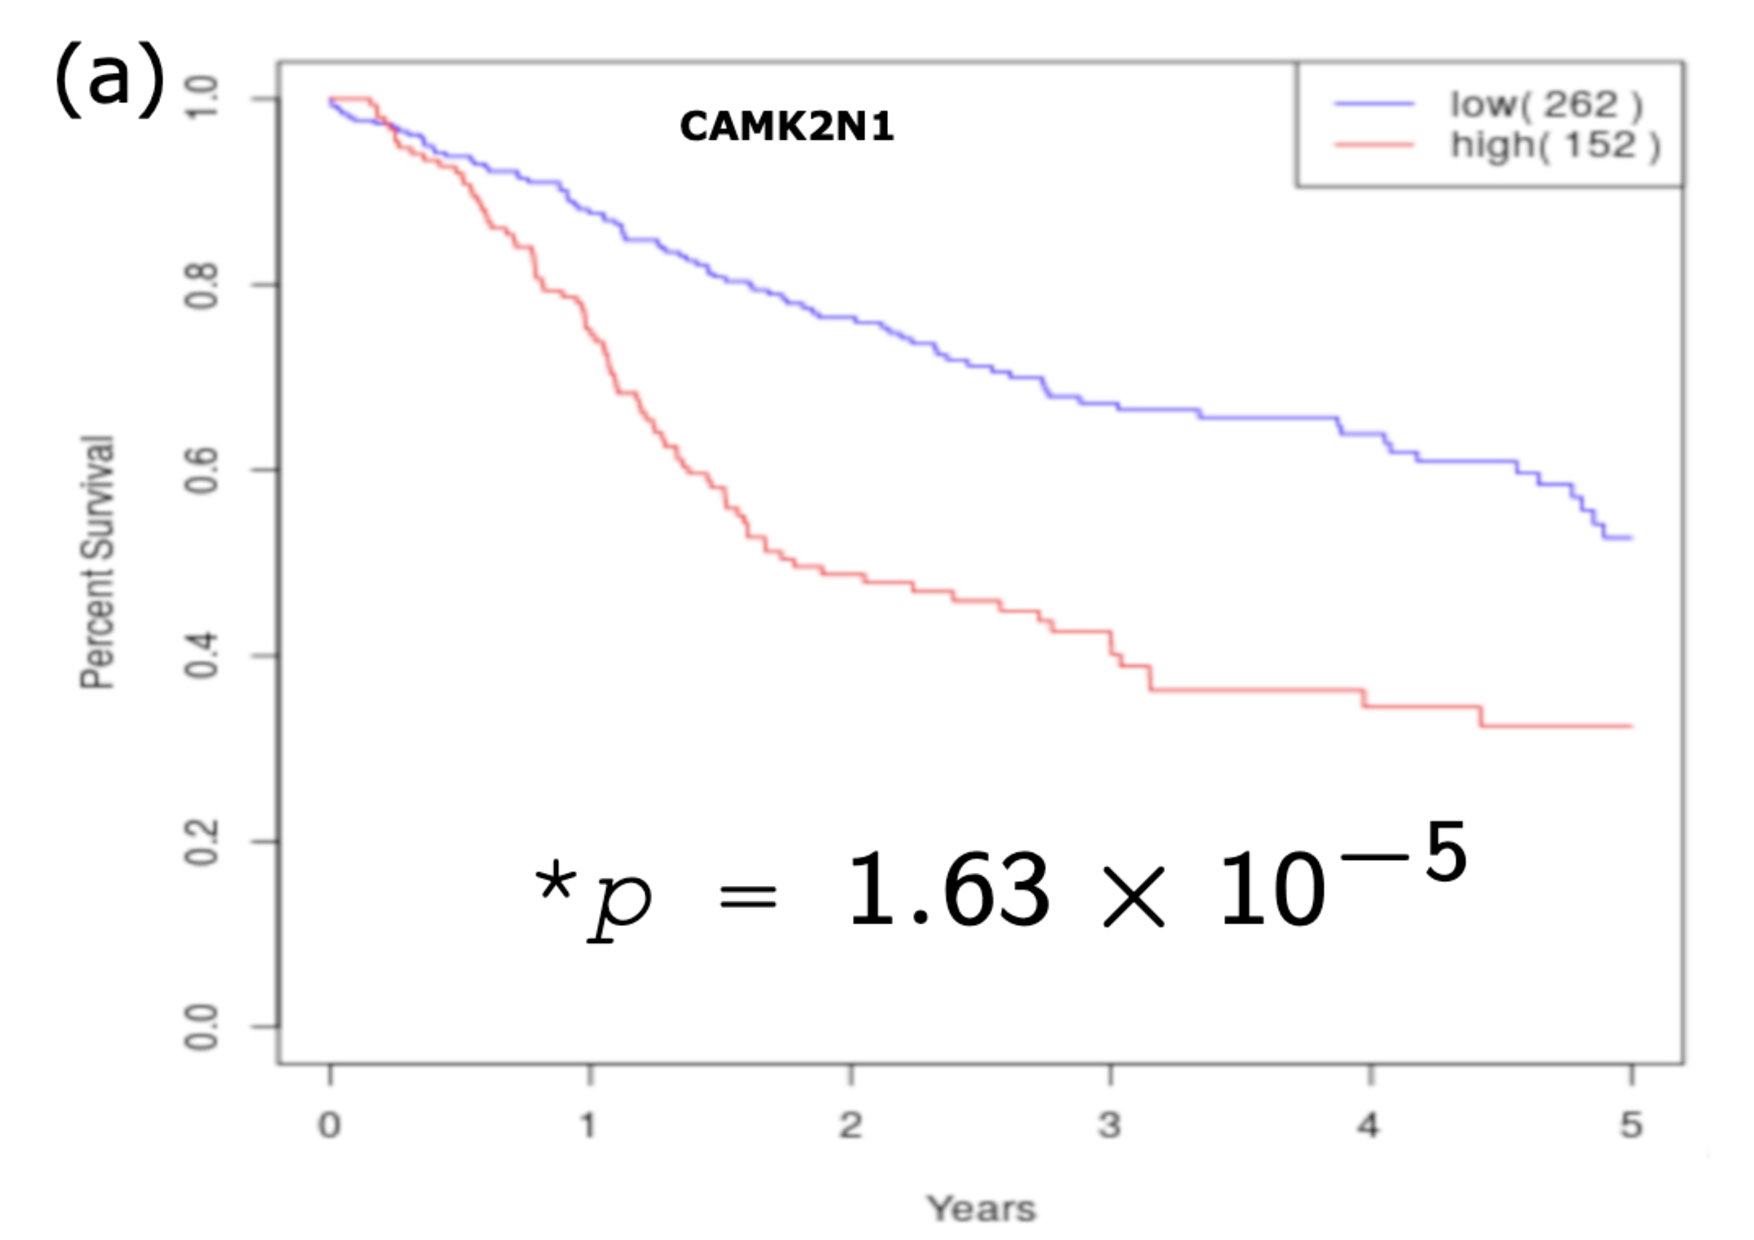
\includegraphics[width=0.95\textwidth]{KMplot_CAMK2N1.pdf}
%\end{minipage}

\end{posterbox}



%%%%%%%
\section{Holistic Cancer Care}
\begin{posterbox}[name=feedback,column=2,below=problems, above=bottom]{Holistic Cancer Care}
Holistic (whole) cancer care~[Mehta, 2019][Iftikhar, 2021]: to care \underline{spirit}, \underline{emotion}, \underline{the body} of a person, and his \underline{social} relation.

%%
\begin{center}
  \includegraphics[width=0.9\textwidth]{Figure_5_holisticCare.pdf}
\end{center}
%\includegraphics[width=10cm]{Figure_5_holisticCare.pdf}

 
\begin{outline}
\1 to give the physical care: systemic therapy (drug) or surgery
%\1 to support cancer patients' spiritual, emotional, physical, and socioeconomic needs

\1 \underline{therapeutic relationship}~[Rogers, 1979], the physicians' spiritual properties \underline{(empathy, sympathy, and compassion)} will engage cancer patients
\1 to induce their \underline{self-compassion} to gain \underline{resilience against} the disease through their mind--brain--body axis~[Hsiao, 2012]
\1 to reduce pain, to promote survival from cancer

\end{outline}

\end{posterbox}



%%%% Reference no more reference
%\begin{posterbox}[name=refs,column=2,below=feedback,above=bottom]{References}
% In the last box, you will usually have a list of references
% The bibliography automatically adds the title "References", but
% this have been removed in the preamble



% use either ......
%\bibliographystyle{plain}
%\bibliography{TCGA_margin_cutoff.bib}



% ...... or
%  \bibliographystyle{IEEEbib}
%  \bibliography{IEEEabrv,mybib,mybib2} 
%\end{posterbox}

\end{poster}
\end{document}


%%%%%%%%%%%%%%%%%%%%% spared code
\begin{thebibliography}{1}% Simple bibliography with widest label of 1
\itemsep=-0.01em% Save space between the separation
\setlength{\baselineskip}{0.4em}% Save space with longer lines
\bibitem{baposter} Brian Amberg: \emph{LaTeX Poster Template}, \url{http://www.brian-amberg.de/uni/poster/} 
\bibitem{pgfplots} Christian Feuersänger: \emph{PGFPlots - A LaTeX Package to create normal/logarithmic plots in two and three dimensions}, \url{http://pgfplots.sourceforge.net/} 
\bibitem{jknaau} Jesper Kjær Nielsen: \emph{Official AAU Beamer Theme, Poster Theme, and Report Template}, \url{http://kom.aau.dk/~jkn/latex/latex.php}
\bibitem{jknsqrt-1} Jesper Kjær Nielsen: \emph{Official AAU Beamer Theme, Poster Theme, and Report Template}, \url{http://sqrt-1.dk/latex/latex.php}
\end{thebibliography}

%
%\begin{posterbox}[name=usage,column=0,below=intro]{Usage}
\begin{itemize}
  \item To use the AAU poster theme, place the {\tt aauposter.tex} file in your preferred folder and modify the file to your needs.
  \item You can read more about how you can modify the theme in the documentation for the baposter template which you can find here \url{http://www.brian-amberg.de/uni/poster/}.
\end{itemize}


%%

Itemize
\begin{itemize}
  \item item 1
    \begin{itemize}
      \item subitem 1
        \begin{itemize}
          \item subsubitem 1
            \begin{itemize}
              \item subsubsubitem 1
              \item subsubsubitem 2
            \end{itemize}
          \item subsubitem 2
        \end{itemize}
      \item subitem 2
    \end{itemize}
  \item item 2
\end{itemize}
Enumerate
\begin{enumerate}
  \item item 1
    \begin{enumerate}
      \item subitem 1
        \begin{enumerate}
          \item subsubitem 1
            \begin{enumerate}
              \item subsubsubitem 1
              \item subsubsubitem 2
            \end{enumerate}
          \item subsubitem 2
        \end{enumerate}
      \item subitem 2
    \end{enumerate}
  \item item 2
\end{enumerate}
Description
\begin{description}
  \item[desc 1] item 1
    \begin{description}
      \item[desc 1] subitem 1
        \begin{description}
          \item[desc 1] subsubitem 1
            \begin{description}
              \item[desc 1] subsubsubitem 1
              \item[desc 2] subsubsubitem 2
            \end{description}
          \item[desc 2] subsubitem 2
        \end{description}
      \item[desc 2] subitem 2
    \end{description}
  \item[desc 2] item 2
\end{description}



